\chapter{Introduction}
\label{chap:introduction}



The \emph{language inclusion problem} is a fundamental and classical problem
which consists in deciding, given two languages $L_1$ and $L_2$,
whether $L_1 \subseteq L_2$.
This problem has a wide variety of applications, ranging from
\emph{automata-based verification}~\cite{kupferman2018automata},
reasoning for \emph{logical theories}~\cite{esparza2017automata} to
\emph{type systems}~\cite{hofmann2014abstract}.
Whether the language inclusion problem is computable or not, depends on the nature
of the languages and, also if it turns out to be computable, it is usually
computationally intensive.

We will formally see that a language is ultimately a set of \emph{words},
that are just concatenated symbols from one \emph{alphabet} $\Sigma$.
In general, languages are \emph{not finite}, so that it is not possible to simply
compute all the words in two languages and compare them.
A vast assortment of techniques and algorithms have been proposed in the past
to solve the problem for certain classes of languages
~\cite{ganty2019language,ouaknine2004language,abdulla2011advanced}.
In particular, we are interested in the language inclusion problem between
\emph{$\omega$-regular languages}, that are languages of \emph{infinite words}
recognized by \emph{B{\"u}chi automata}~\cite{cohen1977theory}.
We consider the framework put forward in~\cite{ganty2020omegalang}, that
relies on \emph{abstract interpretation}~\cite{cousot1977abstract} techniques
in order to solve the language inclusion problem.

\begin{figure}[h]
	\centering
	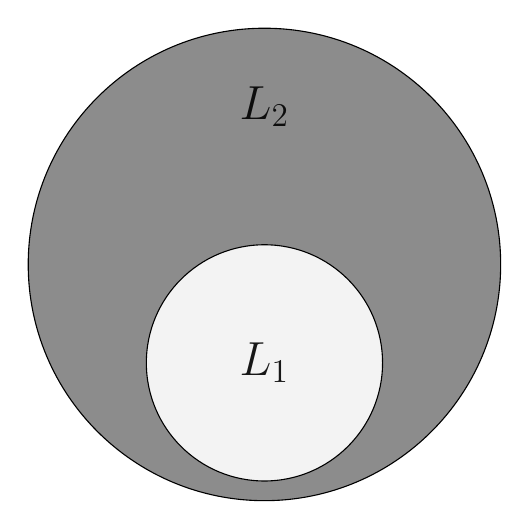
\begin{tikzpicture}
		\begin{scope} [fill opacity = .9]
			\draw[fill=gray, draw = black] (0,0) circle (3);
			\draw[fill=white, draw = black] (0,-1.25) circle (1.5);
			\node at (0,2) {\LARGE\textbf{$L_2$}};
			\node at (0,-1.25) {\LARGE\textbf{$L_1$}};
		\end{scope}
	\end{tikzpicture}
	\caption{Representation of two languages $L_1,L_2$ such that $L_1 \subseteq L_2$}
\end{figure}

The theory of Abstract Interpretation, introduced in~\cite{cousot1977abstract},
is a general theory of the approximation of formal program semantics.
It is an invaluable tool to prove the correctness of a static analysis,
as it makes it possible to express mathematically the link between the
output of a practical, approximate analysis, and the original,
uncomputable program semantics~\cite{mine2017tutorial}.
Although the most well-known application of abstract interpretation theory
is \emph{program verification}~\cite{cousot2005astree},
during the years it has been exploited in
many different fields: from efficient algorithms to compute the simulation
equivalence~\cite{ranzato2007new}, to artificial
intelligence~\cite{ranzato2019robustness}.
Most of the time, the abstractions are \emph{sound} but not \emph{complete},
giving up precision in order to gain decidability.
As we will see, the framework described in~\cite{ganty2020omegalang} is
\emph{sound and complete}, meaning that exactly solves the language inclusion
problem between $\omega$-regular languages, while not raising \emph{false alarms},
as they are known in abstract interpretation terminology.

In particular, the idea is to \emph{abstract} the language $L_1$ with
an \emph{over approximation} function $\rho$.
As long as $\rho$ satisfies a \emph{completeness condition}, that intuitively
corresponds to not losing precision while abstracting the language,
we show how to use $\rho$ in order to checking the inclusion between two languages.

The framework to solve the inclusion between $\omega$-regular languages
described in~\cite{ganty2020omegalang}
is parameterized by a pair of \emph{quasiorders} $\leq_1, \leq_2$ on words:
as long as $\leq_1,\leq_2$ satisfy a list of requirements related to computability
and completeness, they can be plugged into the framework in order to check
the inclusion between two languages.
As one could imagine, the performance of the algorithm described
in~\cite{ganty2020omegalang} depends on the choice of the two quasiorders.
In particular, \emph{coarser} relations lead to algorithms that converge in
less iterations.
They also suggest two families of quasiorders that are suitable for
the described framework: the \emph{syntactic} and the \emph{state-based} quasiorders.
Our ultimate goal is to put forward a number of relations on words that are based on
the \emph{simulation relation} on the states of an automaton.
We explore an ample mix of simulation relations, from the well-known
\emph{direct simulation}~\cite{dill1991checking}, up to less celebrated simulations,
as the \emph{k-lookahead simulation}~\cite{clemente2017efficient}.
We will see that the \emph{simulation-based quasiorders on words} result in
\emph{coarser} relations than the state-based quasiorders, while being
\emph{finer} than the syntactic ones, effectively lying in
the middle between the already proposed relations.

In Chapter~\ref{chap:background} we formally define the concepts that will be
needed in the rest of our work.
We also describe the framework put forward in~\cite{ganty2020omegalang} on
which we rely in order to check the inclusion between $\omega$-regular languages;
in Chapter~\ref{chap:qos} we define various simulation-based quasiorders on words
and we prove that they meet the requirements of the framework, and, finally,
in Chapter~\ref{chap:examples} we give several examples that show the practical
advantages of using the simulation-based quasiorders.
